\documentclass[12pt]{ctexart}
\usepackage{amsmath,graphicx,textcomp,subfigure,indentfirst,ctex,color,float}
\title{Lecture 8}
\author{赵思逸}

\date{2022年4月19日}

\newcommand{\refeq}[1]{式~(\ref{#1})}
\newcommand{\reffig}[1]{图~(\ref{#1})}
\begin{document}

\maketitle

\section*{微波背景辐射(续)}

为什么CMB符合黑体谱?

在最后散射面 $t_L$,光子辐射谱满足Planck公式:
\begin{equation}
    n_{T(t_L)}(\nu_L) d \nu_L=\frac{8 \pi \nu_L^{2} d \nu_L}{\exp \left(\frac{h_\text{pl} \nu_L}{k_{B} T(t_L)} \right)-1}
\end{equation}
在$t>t_L$,光子频率由于宇宙学红移降低 $\nu=\nu_{L} \frac{a(t_L)}{a(t)}$,
光子数密度 $n\left(\nu, t\right) d\nu \propto a^{-3}$即
\begin{equation}
    n(\nu, t) d \nu=\left(\frac{a(t_L)}{a(t)}\right)^{3} n_{T\left(t_{L}\right)}\left(\nu_{L}\right) d \nu_{L}
\end{equation}

代入得
\begin{equation}
    n(\nu, t) d \nu = \frac{8 \pi \nu^{2} d \nu}{\exp \left(\frac{h_\text{pl} \nu}{k_{B} \frac{a(t_L)}{a(t)}T(t_L)}   \right)-1}
\end{equation}
仍然是黑体谱。此时光子不处于热平衡,不妨令$T(t)=\frac{a(t_L)}{a(t)}T(t_L)$,即$T\propto 1/a$.

\subsection*{光子、核子密度}

光子的能量密度 $\rho_\gamma = \int h_{\mathrm{pl}} \nu n(\nu) d\nu = a_B T^4$, 其中 $a_B=\frac{8\pi^5 k_B^4}{15 h_{\mathrm{pl}}^3 c^3 } = 7.566\times 10^{-15} \mathrm{~erg~cm^{-3}K^{-4}}$.

今天 $T_{\gamma,0} = 2.725 \mathrm{K}$, $\rho_{\gamma,0}=a_B T_{\gamma,0}^4 = 4.64\times 10^{-34} \mathrm{~g~cm^{-3}}$,
$\Omega_\gamma = \frac{\rho_{\gamma,0}}{\rho_\text{crit}} = 2.47\times 10^{-5} h^{-2} \simeq 5\times 10^{-5}$.

今天的总辐射包括光子和中微子。中微子作为费米子,和光子的统计不同。且中微子退耦更早,所以温度低于光子。最后,中微子有3种。总结如下
\begin{equation}
    \rho_{R, 0}=\rho_{\gamma, 0}+\rho_{\gamma, 0} \times\left(\frac{7}{8}\right) \times\left(\frac{4}{11}\right)^{4 / 3} \times 3 =7.80 \times 10^{-34} \mathrm{~g~cm^{-3}}
\end{equation}

总之今天辐射的能量密度远远小于冷物质和暗能量。
\begin{equation}
    \begin{aligned}
        \Omega_{R}=\frac{\rho_{R, 0}}{\rho_\text{crit}} &=4.15 \times 10^{-5} h^{-2} \\
        & \simeq 8.3 \times 10^{-5} \ll \Omega_M, \Omega_\Lambda
    \end{aligned}
\end{equation}

考虑光子的数密度
\begin{equation}
    n_{\gamma}=\int_{0}^{\infty} n_{T}(\nu) d \nu=\frac{30 \zeta(3)}{\pi^{4}} \frac{a_{B}}{k_{B}} T^{3}=20.28 T^{3} \mathrm{~cm}^{-3}
\end{equation}

今天 $T_{\gamma,0} = 2.725 \mathrm{K}$, $n_{\gamma, 0}=410$ photons $/ \mathrm{cm}^{3}$

核子数密度
\begin{equation}
    n_{B, 0}=\frac{\rho_{B, 0}}{m_{N}}=\frac{\Omega_{B} \rho_{\text {crit }}}{m_{N}}=1.123 \times 10^{-5} \Omega_{B} h^{2} \text { nucleons } / \mathrm{cm}^{3}
\end{equation}
其中 $m_{N}$ 是核子平均质量。

光子与核子数密度比
% $$
% \frac{n_{\gamma}}{n_{B}}=\frac{n_{\gamma,0}}{n_{B, 0}}=3.65 \times 11^{7} /\left(\Omega_{B} h^{2}\right) \simeq 2.4\times 10^9
% $$
\begin{equation}
    \eta = \frac{n_{B}}{n_{\gamma}} \simeq 4.1\times 10^{-10}
\end{equation}

上节课讲过,在绝热膨胀的宇宙中,为了保持普朗克黑体辐射谱,我们定义非热平衡的光子的温度正比于$a$的$-1$次方。
对于非相对论性粒子,为了遵循玻尔兹曼统计,温度正比于$a$的$-2$次方。
在退耦前,光子和核子处于热平衡,光子远多于核子,占据主导,温度正比于$a$的$-1$次方。

\subsection*{估算光子退耦时刻}

散射速率
\begin{equation}
    \Lambda_\gamma=\sigma_{T} n_{e} c=0.88 n_{B,0}\left(\frac{T}{T_{\gamma,0}}\right)^{3} \sigma_{T} c=1.97 \times 10^{-19} \mathrm{~s}^{-1} \Omega_{\mathrm{B}}{h }^{2}\left(T / T_{\gamma,0}\right)^{3}
\end{equation}

其中用到平均一个核子对应$Y_H+\frac{1}{2}Y_{He}=0.76+\frac{1}{2}\times 0.24=0.88$个电子。

能量转移速率
\begin{equation}
    \Gamma \gamma \simeq\left(\frac{\Delta E}{k_{B} T}\right) \Lambda_{\gamma} \approx\left(\frac{k_{B} T}{m_{e} c^{2}}\right) \Lambda_{\gamma} \simeq 9.0 \times 10^{-29} s^{-1} \Omega_{B} h^{2}\left(\frac{T}{T_{\gamma,{0}}}\right)^{4}
\end{equation}

而宇宙膨胀速率(假设辐射占主导)
\begin{equation}
    \begin{aligned}
        H=\frac{\dot{a}}{a} & \approx H_{0} \sqrt{\Omega_R\left(T / T_{\gamma,{0}}\right)^{4}} \\
    &=2.1\times 10^{-20} s^{-1} \left(\frac{T}{T_{\gamma,{0}}}\right)^{2}
    \end{aligned}
\end{equation}

能量转移速率比膨胀速率下降快,当 $\Gamma_{\gamma} \leq H$ ,散射速率不足,光子与重子物质退耦,也可以叫freeze out.此时温度约为$10^5 \mathrm{~K}$.
但后面会看到,这样估算出的温度过高,处于辐射为主的阶段,是不准确的。

\subsection*{物质-辐射相等时刻}
辐射的能量密度正比于$a$的$-4$次方,冷物质的能量密度正比于$a$的$-3$次方,辐射密度下降快,辐射在宇宙早期先占据主导,后来下降到小于冷物质的能量密度,二者相等的时刻叫做“物质-辐射相等时刻”(matter-radiation equality epoch).
\begin{equation}
    T_{eq}=T_{\gamma,0}\left(\frac{\Omega_{M}}{\Omega_{R}}\right)=6.56 \times 10^{4} \Omega_{m} h^{2} \mathrm{~K} =10^{4} \mathrm{~K}
\end{equation}
一般使用红移表示
\begin{equation}
    1+z_{eq}=\left(\frac{a_{e q}}{a_{0}}\right)^{-1}=\frac{\Omega_{M}}{\Omega_{R}}=2.4 \times 10^{4}\left(\Omega_M h^{2}\right) \simeq 3500
\end{equation}

\subsection*{Boltzmann方程和Saha方程}
对于反应 $1+2 \longleftrightarrow 3+4$,
非平衡态下的Boltzmann方程为
\begin{equation}
    a^{-3} \frac{d}{d t}\left(n_{1} a^{3}\right)=n_{1}^{(0)} n_{2}^{(0)}\langle\sigma v\rangle\left(\frac{n_{3} n_{4}}{n_{3}^{(0)} n_{4}^{(0)}}-\frac{n_{1} n_{2}}{n_{1}^{(0)} n_{2}^{(0)}}\right)
\end{equation}
其中 $\langle\sigma v\rangle$ 是 thermally averaged cross-section. 括号中第一项度量了反应向左移动的速率,第二项度量了反应向右移动的速率。
\begin{equation}
    n_{i}^{(0)}=\left\{\begin{array}{l}
    g_{i}\left(\frac{m_i T}{2 \pi}\right)^{3 / 2} e^{-\frac{m_{i} c^{2}}{k_{B} T}  }, \qquad m_{i} c^{2}\gg k_{B} T \\
    \frac{g_{i}^{3}}{\pi^{2}}T^3, \qquad m_{i} c^{2}\ll k_{B} T 
    \end{array}\right.
\end{equation}

平衡态下的精细平衡方程
\begin{equation}
    \frac{n_{3} n_{4}}{n_{3}^{(0)} n_{4}^{(0)}}=\frac{n_{1} n_{2}}{n_{1}^{(0)} n_{2}^{(0)}}
\end{equation}

具体到再复合(recombination),反应是 $e+p \leftrightarrow H+\gamma$.
代入精细平衡方程得到Saha方程
\begin{equation}
    \frac{n_{e}n_p}{n_{H}}=\frac{n_{e}^{(0)} n_{p}^{(0)}}{n_{H}^{(0)}}
\end{equation}

其中光子的化学势为0,$n_\gamma = n_{\gamma}^{(0)}$.
忽略He贡献,电子数密度与质子数密度近似相等
$$n_{e}=n_{p}=X_{e} n_{b}$$
其中$n_{b}=n_{p}+n_{H}$ 是重子数密度,$X_e$ 是电离度。剩下的H以中性原子形式存在
$$n_{H}=\left(1 - X_{e}\right) n_{b}$$

此时温度远小于质子和电子的能标,使用非相对论情形计算$n_i^{(0)}$
\begin{eqnarray}
      \frac{n_{e}^{(0)} n_{p}^{(0)}}{n_{H}^{(0)}} &=& \frac{g_e g_p}{g_H} \left(\frac{m_e m_p}{m_H}\right)^\frac{3}{2} \left(\frac{T}{2\pi }\right)^\frac{3 }{2} e^{-\frac{B_1}{k_B T}} \\ 
      &\simeq&\left(\frac{m_e T}{2\pi }\right)^\frac{3 }{2} e^{-\frac{B_1}{k_B T}}
\end{eqnarray}

  
其中 $B_1=m_e+m_p - m_H=13.6\mathrm{eV}$ 是中性氢原子的结合能, 自由度 $g_e=2,g_p=2,g_H=4$.

Boltzmann方程左边
\begin{equation}
    a^{-3} \frac{d}{d t}\left(n_{e} a^{3}\right)= a^{-3} \frac{d}{d t}\left(X_{e} n_{b} a^{3}\right) = n_b \frac{d X_e}{dt}
\end{equation}

即
\begin{eqnarray}
    n_b \frac{d X_e}{dt} &=& n_{e}^{(0)} n_{p}^{(0)}\langle\sigma v\rangle\left(\frac{n_H}{n_{H}^{(0)}}-\frac{n_{e} n_{p}}{n_{e}^{(0)} n_{p}^{(0)}}\right)   \\ 
    &=& (1-X_e) n_b \langle\sigma v\rangle \frac{n_{e}^{(0)} n_{p}^{(0)}}{n_H^{(0)}} - X_e^2 n_b^2 \langle\sigma v\rangle \\
    &=& (1-X_e) n_b \beta  - X_e^2 n_b^2 \alpha^{(2)}
\end{eqnarray}
其中
\begin{equation}
    \beta \equiv \langle\sigma v\rangle\left(\frac{m_{e} T}{2 \pi}\right)^\frac{3 }{2} e^{-\frac{B_1}{k_B T}}
\end{equation}
\begin{equation}
    \alpha^{(2)} \equiv \langle\sigma v\rangle=9.78 \frac{\alpha^{2}}{m_{e}^{2}}\left(\frac{B_{1}}{k_{B} T}\right)^\frac{1 }{2} \ln \left(\frac{B_{1}}{k_{B} T}\right)
\end{equation}

得到Boltzmann方程
\begin{equation}
    \frac{d X_{e}}{d t}=\left(1-X_{e}\right) \beta-X_{e}^{2} n_{b} \alpha^{(2)}
\end{equation}

再复合开始时,$\frac{d X_{e}}{d t}=0$, $\text{RHS}=0$,即Saha方程
\begin{equation}
    \frac{X_{e}^{2}}{\left(1-X_{e}\right)} = \frac{\beta}{n_{b} \alpha^{(2)}} = \frac{1 }{n_b} \left(\frac{m_{e} T}{2 \pi}\right)^\frac{3 }{2} e^{-\frac{B_1}{k_B T}}
\end{equation}
指数项占主导。

解Saha方程的结果是退耦发生在$z\sim 1100$, $T\sim 3000\mathrm{K}$时。

但是Saha方程的解是电离度一直随exp指数下降,这是不准确的。考虑到退耦后平衡态被打破,应使用非平衡态的Boltzmann方程求解,则可以正确地给出退耦后的残余电离度约为$10^{-3}$,见下图(引自Dodelson)。
\begin{figure}[!hbtp]
	\centering
	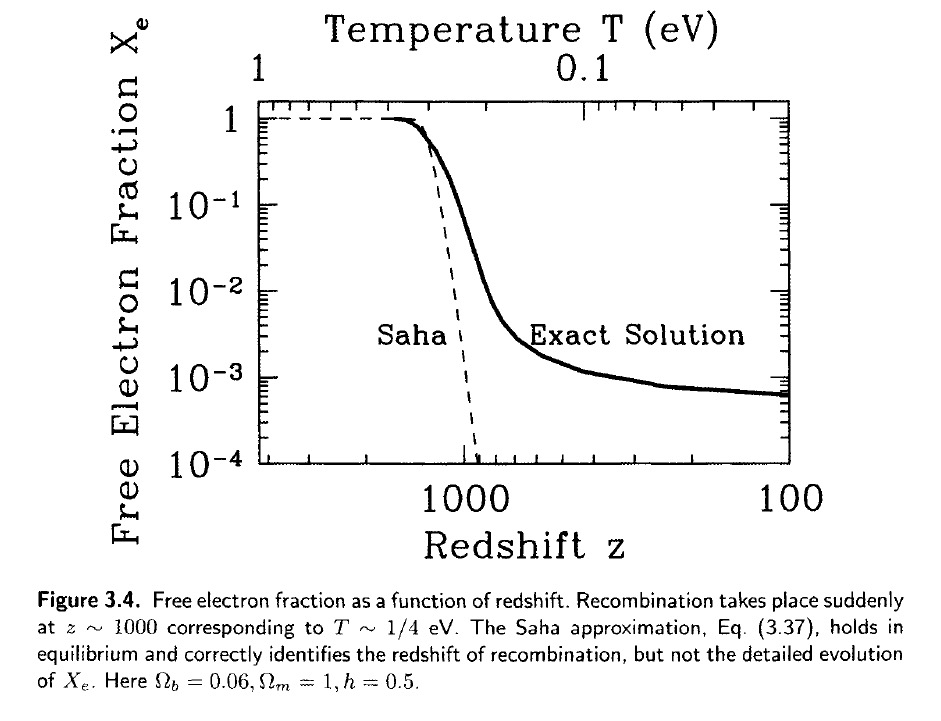
\includegraphics[width=1.0\linewidth]{recombination.jpg}
	\caption{再复合时期电离度的下降} 
\end{figure}


\end{document}
